\documentclass{beamer}
\usepackage{appendixnumberbeamer}

\mode<presentation>{\usetheme[subsectionpage=progressbar,block=fill,numbering=none]{metropolis}}

\usepackage[sfdefault]{FiraSans} %% option 'sfdefault' activates Fira Sans as the default text font
\usepackage[english]{babel} 
% \usepackage[utf8]{inputenc}

\usepackage{graphicx} % Allows including images
\usepackage{caption}
\usepackage{booktabs} % Allows the use of \toprule, \midrule and \bottomrule in tables
\usepackage{multicol} 

% Math packages
\usepackage{amsmath}
\usepackage{mathtools}
\usepackage{amssymb}
\usepackage{mathpartir}

% Lean 
\usepackage[outputdir=build]{minted}
\setminted{encoding=utf-8}
\usepackage{fontspec}
\setmainfont{FreeSerif}
\setmonofont{FreeMono}
\setminted[Lean]{
mathescape=true,
linenos=true,
breaklines=true,
numbersep=5pt,
fontsize=\small,
frame=lines,
framesep=2mm
}

% Coloured boxes
\usepackage{tcolorbox}
\colorlet{alert}{mLightBrown}
\newtcolorbox{alertbox}
{standard jigsaw, opacityback=0,colframe=alert}
\newtcolorbox{tbox}
{standard jigsaw, opacityback=0,opacityframe=0}

\title{Continued Fractions in Lean} % the title on the title page
\subtitle{A Newbie's Adventure}

\author{Kevin Kappelmann} % Your name
\institute[VU Amsterdam]{Vrije Universiteit Amsterdam}
\date{June 14, 2019} % Date, can be changed to a custom date

\begin{document}

\maketitle

%------------------------------------------------
\section{Let's Go on an Adventure}
\begin{frame}{Choose a Weapon}
\pause
\only<2>{\begin{figure}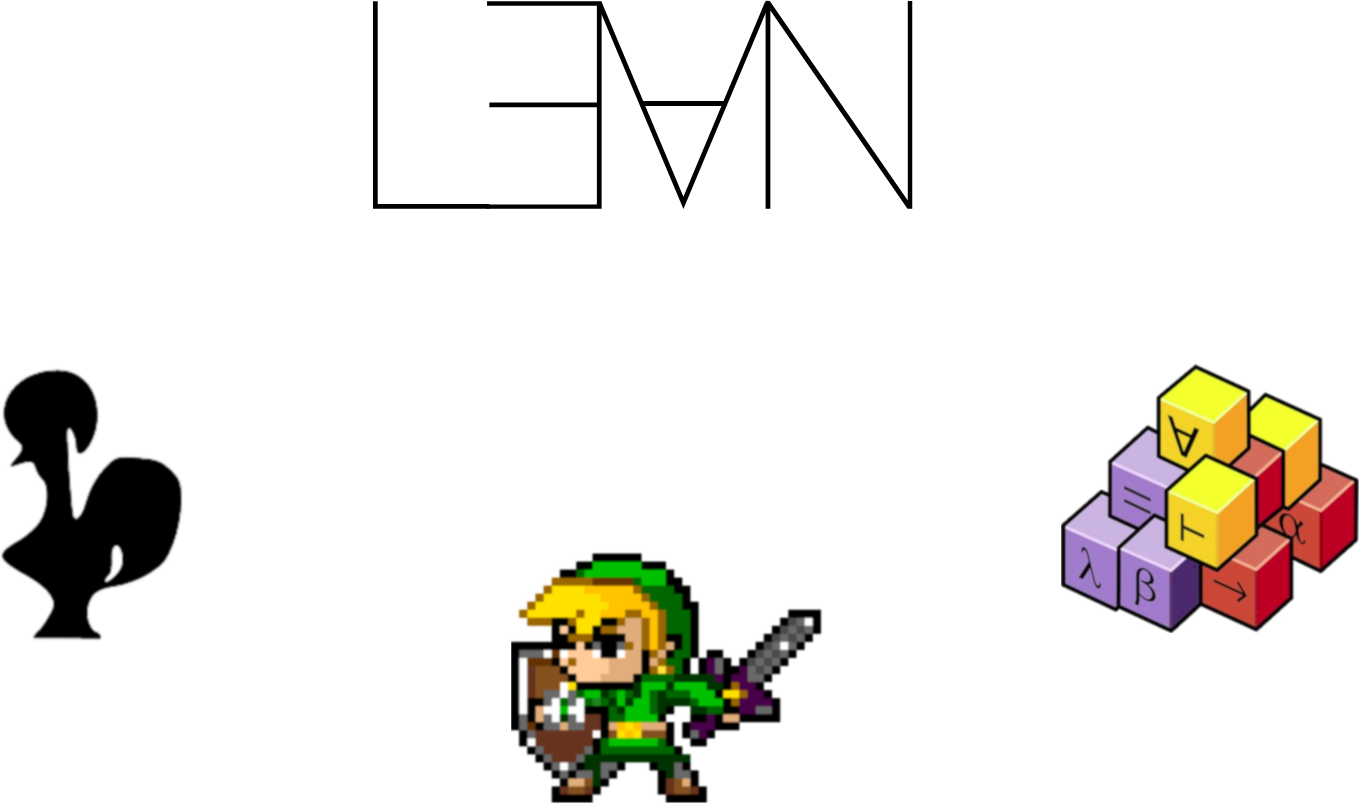
\includegraphics[height=0.6\textheight]{img/choose_prover.png}\end{figure}}
\only<3->{\begin{figure}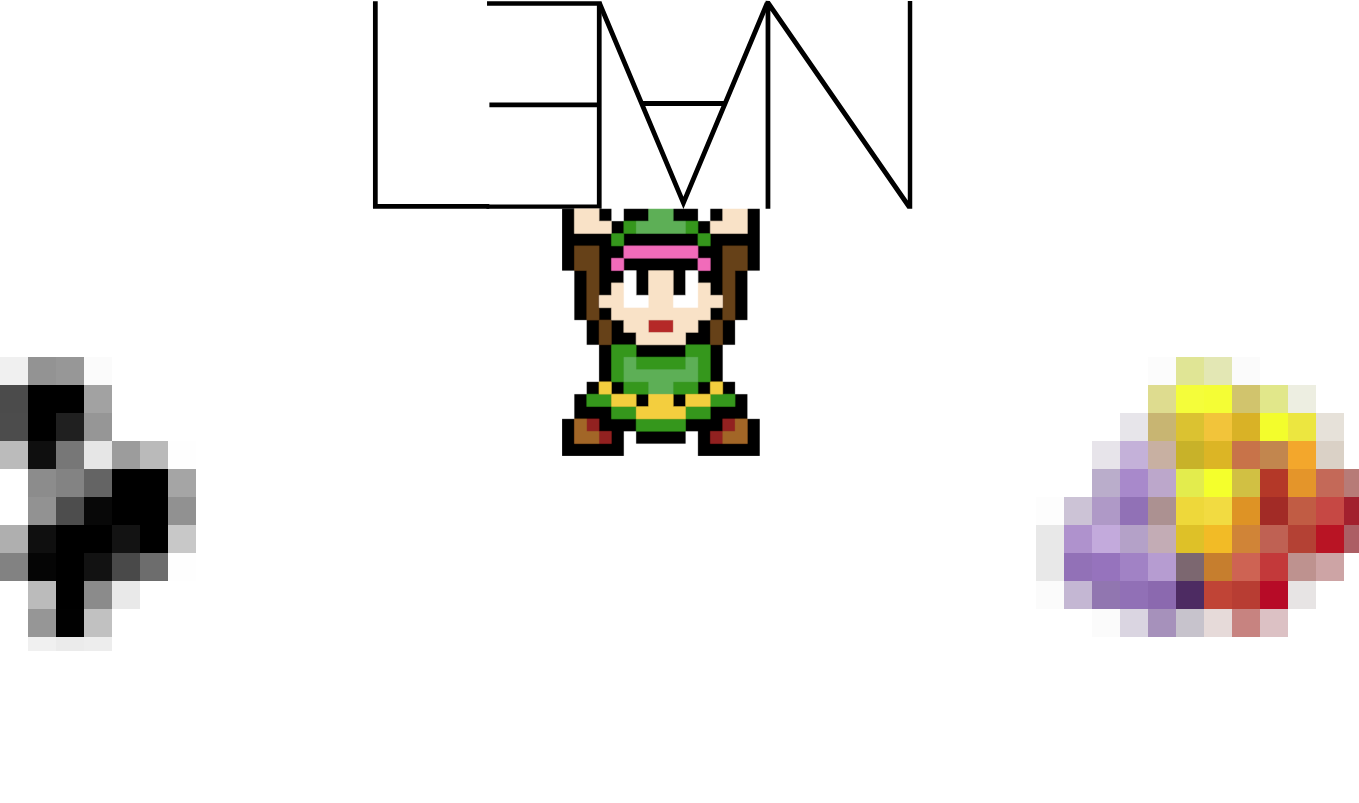
\includegraphics[height=0.6\textheight]{img/choose_prover2.png}\end{figure}}
\visible<4>{
\centerline{\dots perhaps because I am interning at VU Amsterdam}
}
\end{frame}
%------------------------------------------------
\begin{frame}{The Adventurer's Skill Set}
\pause
\begin{itemize}[<+->]
\item Some experience using Isabelle
\item First project with a dependent type theorem prover
\item Basic maths and functional programming knowledge
\end{itemize}
\end{frame}
%------------------------------------------------
\begin{frame}
\begin{figure}
    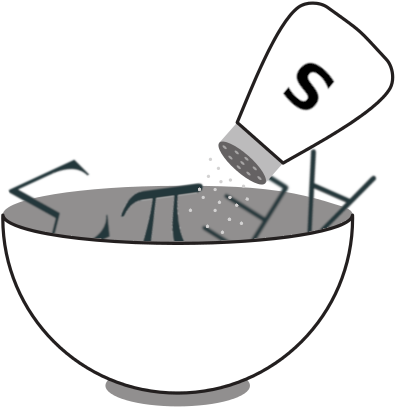
\includegraphics[height=0.8\textheight]{img/salt_shaker.png}
\end{figure}
\end{frame}
%------------------------------------------------
\section{Definitions}
\begin{frame}{Generalized Continued Fractions}
A generalized continued fraction is\dots
\pause
\begin{equation*}
b + \cfrac{a_0}{b_0 + \cfrac{a_1}{b_1 + \cfrac{a_2}{b_2 + \cfrac{a_3}{b_3 + \ddots\,}}}}
\end{equation*}
\pause
\begin{itemize}[<+->]
\item $b$ is called the \emph{integer part}
\item each $a_i$ is a \emph{partial numerator}
\item each $b_i$ is a \emph{partial denominator}
\end{itemize}
\end{frame}
%------------------------------------------------
\begin{frame}{Generalized Continued Fractions of $\pi$}
\begin{columns}
\column{0.49\textwidth}
\visible<2->{
    \only<1-2>{\centerline{\alert{Continued fraction}}}
    \only<3->{\centerline{Continued fraction}}
}
\begin{equation*}
\resizebox{1\hsize}{!}{$
\pi=3+\cfrac{1}{7+\cfrac{1}{15+\cfrac{1}{1+\cfrac{1}{292+\cfrac{1}{1+\ddots}}}}}
$}
\end{equation*}
\column{0.49\textwidth}
\vspace{5.3mm}
\visible<3->{
\visible<4->{
    \centerline{\alert{Generalized continued fraction}}
}
\begin{equation*}
\resizebox{1\hsize}{!}{$
\pi=3+\cfrac{1^2}{6+\cfrac{3^2}{6+\cfrac{5^2}{6+\cfrac{7^2}{6+\cfrac{9^2}{6+\ddots}}}}}
$}
}
\end{equation*}
\end{columns}
\end{frame}
%------------------------------------------------
\begin{frame}[fragile]{Generalized Continued Fractions in Lean}
\begin{columns}
\column{0.30\textwidth}
\begin{equation*}
\resizebox{1\hsize}{!}{$
b + \cfrac{a_0}{b_0 + \cfrac{a_1}{b_1 + \cfrac{a_2}{b_2 + \cfrac{a_3}{b_3 + \ddots\,}}}}$
}
\end{equation*}
\pause
\column{0.65\textwidth}
\begin{onlyenv}<4->
    \begin{minted}[fontsize=\tiny,linenos=false]{Lean}
    /- Fix a type -/
    variable (α : Type*)

    /-- A gcf_pair consists of a partial numerator a and partial denominator b -/
    structure gcf_pair := (a : α) (b : α)
    \end{minted}   
\end{onlyenv}
\end{columns}
\begin{onlyenv}<1-2>
\begin{visibleenv}<2>
\begin{minted}{Lean}
/- Fix a type -/
variable (α : Type*)
\end{minted}
\end{visibleenv}
\end{onlyenv}
\begin{onlyenv}<3>
    \begin{minted}{Lean}
    /- Fix a type -/
    variable (α : Type*)

    /-- A gcf_pair consists of a partial numerator a and partial denominator b -/
    structure gcf_pair := (a : α) (b : α)
    \end{minted}   
\end{onlyenv}
\begin{onlyenv}<4>
\begin{minted}[linenos=false]{Lean}
-- Once a sequence hits none, it stays none
def seq := {f : ℕ → option α // ∀ {n}, f n = none → f (n + 1) = none}
\end{minted}
\end{onlyenv}
\begin{onlyenv}<5>
\begin{minted}[linenos=false]{Lean}
def seq := {f : ℕ → option α // ∀ {n}, f n = none → f (n + 1) = none}
/-- A generalized continued fraction consists of a leading head term (the "integer part") and a sequence of partial partial numerators $a_n$ and partial denominators $b_n$ -/
structure gcf := (head : α) (seq : seq (gcf_pair α))
\end{minted}
\end{onlyenv}
\end{frame}
%------------------------------------------------
\begin{frame}[fragile]{Evaluate Generalized Continued Fractions}
\begin{onlyenv}<1>
\begin{minted}[fontsize=\small]{Lean}
def convergents (g : gcf α) (n : ℕ) : α :=
g.head + if n = 0 then 0 else aux n g.seq
\end{minted}
\end{onlyenv}
\begin{onlyenv}<2>
\begin{minted}[fontsize=\small]{Lean}
def aux : ℕ → seq (gcf_pair α) → α
| 0 s := match s.head with
  | none := 0
  | some ⟨a, b⟩ := a / b
  end
| (n + 1) s := match s.head with
  | none := 0
  | some ⟨a, b⟩ := a / (b + aux n s.tail)
  end

def convergents (g : gcf α) (n : ℕ) : α :=
g.head + if n = 0 then 0 else aux n g.seq
\end{minted}
\end{onlyenv}

\end{frame}
%------------------------------------------------
\begin{frame}[fragile]{Continued Fractions}
\begin{equation*}
\resizebox{0.4\hsize}{!}{$
b + \cfrac{1}{b_0 + \cfrac{1}{b_1 + \cfrac{1}{b_2 + \cfrac{1}{b_3 + \ddots\,}}}}$
}
\end{equation*}
\pause
\vspace{-5mm}
\begin{visibleenv}<2->
\begin{minted}{Lean}
/-- A continued fraction is a gcf whose partial numerators are equal to 1. -/
def cf := {g : gcf α // ∀ (n : ℕ) (a : α), (partial_numerators g).nth n = some a → a = 1}
\end{minted}
\end{visibleenv}
\visible<3-4>{\centerline{First impression: \visible<4>{\alert{Pretty Sweet!}}}}
\end{frame}
%------------------------------------------------
\begin{frame}[fragile]{Fun with Subtypes}
So, since \emph{cf} is a subtype of \emph{gcf}, we can do
\begin{onlyenv}<1-4>
\begin{minted}{Lean}
def convergents (g : gcf α) (n : ℕ) : α := ...

variable (c : cf α)
#check convergents c 0
\end{minted}
\visible<2->{
    \only<1-2>{\textcolor{red}{\centerline{\Large{NOPE!}}}}
    \only<3-4>{\begin{center}{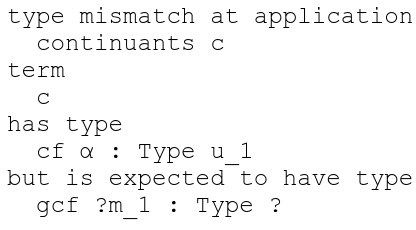
\includegraphics[height=0.4\textheight]{img/subtype_error.png}}\end{center}}
    \visible<4>{\centerline{\alert{Oh, I see -- I need to cast!}}}
}
\end{onlyenv}
\begin{onlyenv}<5->
\begin{minted}{Lean}
def convergents (g : gcf α) (n : ℕ) : α := ...

variable (c : cf α)
#check convergents (c : gcf α) 0
\end{minted}
\visible<6->{
    \only<5-6>{\textcolor{red}{\centerline{\Large{NOPE!}}}}
    \only<7->{\begin{center}{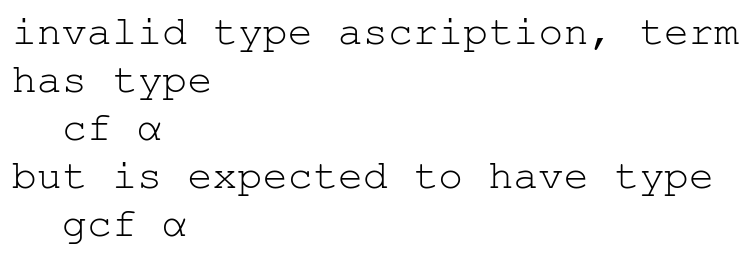
\includegraphics[height=0.3\textheight]{img/subtype_error2.png}}\end{center}}
    \visible<8->{\centerline{\alert{\dots alright, let's go on Zulip 
\includegraphics[height=0.04\textheight]{img/zulip.png}}}}
}
\end{onlyenv}
\end{frame}
%------------------------------------------------
\begin{frame}{Please Help Me}
    \center A few minutes and messages from \href{http://wwwf.imperial.ac.uk/~buzzard/}{\emph{Kevin Buzzard}} later\dots
\end{frame}
%------------------------------------------------
\begin{frame}[fragile]{The ``Solution''}
We first need to define the casting
\pause
\begin{minted}{Lean}
instance cf_to_gcf : has_coe (cf β) (gcf β)
:= by {unfold cf, apply_instance}

/- Best practice: create a lemma for your cast -/
@[simp, elim_cast]
lemma coe_cf (c : cf β) : (↑c : gcf β) = c.val
:= by refl
\end{minted}
\begin{visibleenv}<3->
\begin{onlyenv}<1-3>
\alert{Now this works:}
\begin{minted}{Lean}
variable (c : cf α)
#check convergents (c : gcf α) 0
\end{minted}
\end{onlyenv}
\begin{onlyenv}<4->
\textcolor{red}{This, however, still does not work:}
\begin{minted}{Lean}
variable (c : cf α)
#check convergents c 0
\end{minted}
\end{onlyenv}
\end{visibleenv}
\end{frame}
%------------------------------------------------
\section{Proofs}
%------------------------------------------------
\begin{frame}[fragile]{The Proof Is Trivial}
\begin{minted}{Lean}
lemma floor_rat_eq_num_div_denom (n d : ℤ) :
  ⌊rat.mk n d⌋ = n / d
\end{minted}

\vspace{10mm}
\only<2>{\centerline{Wait, let's do some examples first\dots}}
\only<3>{\centerline{\alert{Alright, I am sold!}}}
\end{frame}
%------------------------------------------------
\begin{frame}[fragile]{Proving\dots\ Please Wait}
\only<1>{\begin{figure}{
\includegraphics[height=0.5\textheight]{img/clock.png}}\end{figure}}
\only<2>{
\begin{figure}{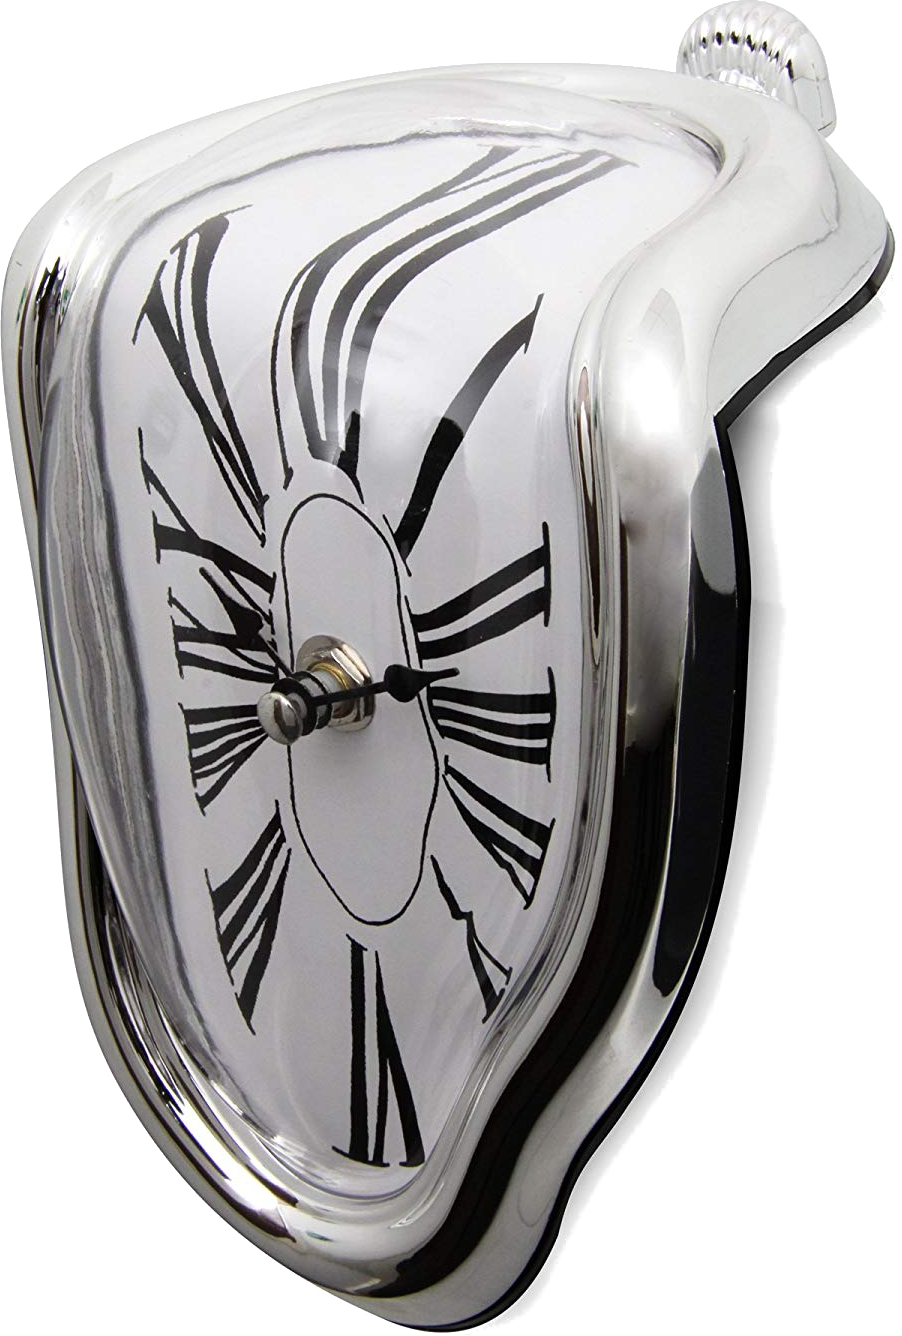
\includegraphics[height=0.5\textheight]{img/melting_clock.png}}\end{figure}

\vspace{5mm}
\centerline{\alert{Something seems wrong}}
}
\end{frame}
%------------------------------------------------
\begin{frame}[fragile]{Now It Is Trivial}
\begin{minted}{Lean}
lemma floor_rat_eq_num_div_denom (n : ℤ) (d : ℕ) :
  ⌊rat.mk n d⌋ = n / d
\end{minted}
\vspace{5mm}
\centerline{That's better!}
\end{frame}
%------------------------------------------------
\begin{frame}[fragile]{A Short Note About Tactics}
\centerline{\emph{<Show two short examples in VS Code>}}
\end{frame}
%------------------------------------------------
\section{Results}
\begin{frame}[fragile]{Collected Treasures}
\only<1>{\begin{figure}
\includegraphics[height=0.6\textheight]{img/chest.png}\end{figure}}
\begin{onlyenv}<2>
Definition of (generalized) continued fractions and their evaluation
\begin{minted}{Lean}
structure gcf := (head : α) (seq : seq (gcf_pair α))
def cf := {g : gcf α // ∀ (n : ℕ) (a : α), (partial_numerators g).nth n = some a → a = 1}
def convergents (g : gcf α) (n : ℕ) : α := ...
\end{minted}
\end{onlyenv}
\begin{onlyenv}<3-4>
Computable continued fractions for discrete linear ordered floor fields 
\begin{minted}{Lean}
def get_cf [discrete_linear_ordered_field α] [floor_ring α] (v : α) : cf α := ...
\end{minted}
\visible<4>{\centerline{Also works for $\mathbb{R}$ -- just not computable\dots}}
\end{onlyenv}
\begin{onlyenv}<5-7>
Termination proof for archimedian fields
\begin{minted}{Lean}
theorem termination_iff_rat [archimedean α] (v : α) :
  Terminates (get_gcf v) ↔ ∃ (q : ℚ), v = (q : α)
\end{minted}
\visible<6-7>{Including a theorem a mathematician would never prove:}
\begin{visibleenv}<7>
\begin{minted}{Lean}
theorem translate_rat_get_cf {q : ℚ}
(v_eq_q : v = q) :
  ((get_gcf q : gcf ℚ) : gcf α) = get_gcf v :=
\end{minted}
\end{visibleenv}
\end{onlyenv}
\begin{onlyenv}<8>
Finite correctness of the computation
\begin{minted}{Lean}
theorem get_gcf_finite_correctness
(terminates: Terminates (get_gcf v)) :
  ∃ (n : ℕ), v = convergents (get_gcf v) n
\end{minted}
\end{onlyenv}
\begin{onlyenv}<9-10>
Some interesting inequalities, and finally:
\begin{minted}{Lean}
theorem epsilon_convergence : ∀ (ε > (0 : α)),
  ∃ (N : ℕ), ∀ (n ≥ N),
  |v - convergents (get_gcf v) n| < ε :=
\end{minted}

\vspace{5mm}
\visible<10>{\centerline{But sadly no library for sequence limits in Lean :(}}
\end{onlyenv}
\end{frame}
%------------------------------------------------
\section{End of the Story}
%------------------------------------------------
\begin{frame}{Lessons Learnt}
\pause
\begin{itemize}[<+->]
\item Lean's type system is very expressive and great for definitions\dots
\begin{itemize}
\item \dots if one knows the gotchas.
\end{itemize}
\item Support on Zulip is fantastic.
\item Existing tactics help a LOT\dots
\begin{itemize}
\item \dots but no integration of automated theorem provers yet.
\end{itemize}
\end{itemize}
\end{frame}
%------------------------------------------------
\begin{frame}{We Need You!}
\Large
\centerline{\alert{Help us making interactive theorem proving}}

\centerline{\alert{an even better place!}}

\end{frame}
%------------------------------------------------
\begin{frame}[standout]
\normalsize{Formalisation can be found at \url{github.com/kappelmann/lean-continued-fractions}}
\pause
\center
% \Large{Thanks for your attention! Any questions?}
\begin{equation*}
Thanks + \cfrac{1}{for + \cfrac{1}{your + \cfrac{1}{attention!}}}
\end{equation*}

\vspace{10mm}

\pause
\Large{\alert{Any questions?}}
\end{frame}
%----------------------------------------------------------------------------------------
%\begin{frame}[allowframebreaks]{References}
  %\bibliography{../paper/sources.bib}
  %\bibliographystyle{abbrv}
%\end{frame}

\begin{frame}[allowframebreaks]{Image Sources}
\begin{itemize}
\item Salt shaker: Modified from \url{bit.ly/2K8Jw8s}
\item Link 1: \url{bit.ly/2wMGOwE}
\item Link 2: \url{bit.ly/2RaypfX}
\item Link 3: \url{bit.ly/2MNGUPt}
\item Clock: \url{bit.ly/2HOc9GC}
\item Melting clock: \url{bit.ly/2MKWknv}
\end{itemize}
\end{frame}

\end{document} 
